\documentclass[12pt]{article}
\usepackage[utf8]{inputenc}
\usepackage{tikz}
\usepackage{amsmath,amsfonts,amssymb,amsthm}
\usepackage[vlined, ruled]{algorithm2e}
\usepackage{geometry}
\usepackage[noend]{algpseudocode}
\usetikzlibrary{bayesnet}
\usepackage[nottoc,numbib]{tocbibind}
\setlength{\parskip}{1em}
\geometry{letterpaper,left=1.5in,right=1in,top=1in,bottom=1in}
\setlength\parindent{0pt}
\linespread{1.5}
\newcommand{\E}{\mathrm{E}}
\newcommand{\Var}{\mathrm{Var}}
\newcommand{\N}{\mathcal{N}}
\newcommand{\tr}{tr}
\newcommand{\matlab}{{\sc Matlab}\ }
\newcommand{\argmax}{\operatornamewithlimits{argmax}}
\newcommand{\insertfigure}{\begin{figure}\caption{A figure caption}\end{figure}}
\makeatletter
\renewcommand\listoffigures{%
    \section{\listfigurename}% Used to be \section*{\listfigurename}
      \@mkboth{\MakeUppercase\listfigurename}%
              {\MakeUppercase\listfigurename}%
    \@starttoc{lof}%
    }
\makeatother

\begin{document}
\pagenumbering{gobble}
{\centering
  \textbf{Dynamic Covariances in Time Sequence Data}\par
  A Thesis\par
  Submitted to the Faculty\par
  in partial fulfillment of the requirements for the\par
  degree of\par
  Master of Science\par
  in\par
  Computer Science\par
  by\par
  Hao Chang\par
  DARTMOUTH COLLEGE\par
  Hanover, New Hampshire\par
  May, 2017\par
}
\vspace{5mm}
\setlength{\parskip}{0em}
\begin{flushright}
Examining Committee:\par
\vspace{5mm}
$\rule{5cm}{0.15mm}$\par
Hany Farid\par
\vspace{5mm}
$\rule{5cm}{0.15mm}$\par
Qiang Liu\par
\vspace{5mm}
$\rule{5cm}{0.25mm}$\par
Jeremy Manning\par
\end{flushright}
\setlength{\parskip}{1em}




\newpage
\null\par
\newpage






\pagenumbering{roman}
\section{Abstract}
High dimensional time sequence data that seem highly random at first glance can intrinsically be structured processes with covariance that changes over time (dynamic covariance). Discovery and analysis of the dynamic covariances behind time sequence data can not only help us understand underlying patterns, but also give us insight into the inherent connections between the events represented by the data. In order to accurately recover dynamic covariances from time sequence data, we present the Time Sequence Covariance Recovery (TimeCorr) method. TimeCorr first approximates covariance fragments at each time point using a fixed range of neighboring time points, then calculates the covariance at each time point $t$ by finding the sum of the Gaussian average over the covariance fragments centering at time point $t$. To illustrate the effectiveness of TimeCorr, we compared its performance with that of the more probabilistic Multivariate Gaussian Process approach and other deterministic covariance recovery techniques. We show that TimeCorr produces more accurate and more stable results across all of our test cases.
\newpage
\section{Acknowledgements}
I would first like to thank my mentors Professor Qiang Liu of the Computer Science Department at Dartmouth College and Professor Jeremy Manning of the Psychological and Brain Sciences Department at Dartmouth College. Professor Liu and Professor Manning were great inspirations for me throughout this project. Their deep understanding of their respective fields and constant flow of bright ideas really expanded my understanding of what it means to love and excel at what I want to do. Professor Liu and Professor Manning provided timely guidance whenever I was in need and constantly encouraged me to try out new ideas and to reach for higher standards. \par

I would also like to thank Professor Hany Farid of the Computer Science Department at Dartmouth College. Professor Farid kindled my first spark of interest in Computer Science and pushed me to pursue graduate education at Dartmouth. He has been a role model for me throughout my five years at Dartmouth and will always be an inspiration for me in my future pursuits in life.\par

I would also like to acknowledge Dilin Wang, Jun Han and Yihao Feng in the DartML laboratory of the Computer Science Department at Dartmouth College. Their door were always open whenever I ran into technical difficulties or had questions about my research or writing.\par

Finally, I must express my very profound gratitude to my parents for providing me with unfailing support and continuous encouragement throughout my years of study and through the process of researching and writing this thesis. This accomplishment would not have been possible without them. Thank you.\par
\newpage
\tableofcontents
\newpage
\listoffigures
\newpage






\pagenumbering{arabic}
\section{Introduction} \label{introduction}
High dimensional time sequence data that seem very random on the surface can have underlying dynamic covariances that intricately weaves structure and connection into variable behaviors. Finding these dynamic covariances can give us insight into patterns in the data, which has practical values in many different areas including finance, economics, brain science, mathematics, etc. However, two major problems inhibit the traditional covariance formula from effectively recovering dynamic covariances:\par
Problems:\par
\begin{enumerate}
\item Finding covariance using data over long time ranges decreases focus on the time point of interest
\item Finding covariance using data within short time ranges introduces instability in estimation and are often inaccurate due to lack of data
\end{enumerate}
To address these problems, we employed the Multivariate Gaussian Process (MGP) approach---a very traditional Bayesian Machine Learning model. However, the probabilistic model was overly computationally intensive and gave very poor performance in recovering dynamic covariances from our synthetic time sequence datasets. Shifting our focus, we decided to explore deterministic methods for the solution. Finding inspiration directly from the covariance formula
\begin{align}
cov(x,y) = \frac{1}{N}\sum_{i=1}^N (x_i - E(X))\cdot(y_i-E(Y))
\end{align}
and partially incorporating the intrinsic structure of the MGP model, we designed the Naive TimeCorr method by applying Gaussian averaging in our covariance formula. This method addresses the lack of locality in the covariance formula by increasing the influence of time points that are closer to our center of interest. Although the results were slightly better than that of our MGP approach, the recovered dynamic covariances were highly unstable with underwhelming accuracy. Finally, we decided to modify the structure of our formula to put even more emphasis on locality. To achieve this, we estimated covariance fragments at each time point using a tight neighborhood of adjacent points, then applied Gaussian averaging over these covariance fragments to integrate information from the rest of the dataset. This is our TimeCorr method. To illustrate our approach, we generated synthetic datasets with underlying dynamic covariances. We demonstrate that TimeCorr is able to accurately recover the dynamic covariances under our synthetic dataset and show that the results significantly improved compared our previous efforts.


\section{Model Descriptions}
\subsection{The Problem}\label{theProblem}
Given a time sequence dataset of dimensions $T\times V$, we put it into the framework of a Multivariate Gaussian Process with number of variables $V$, number of time points $T$, and underlying dynamic covariance $C_t$ at time $t$. At every time point $t$, the covariance $C_t$ is a square matrix of dimensions $V \times V$, with the element $C^{ij}_T$ at the $i^{th}$ row and $j^{th}$ column representing the joint variability of variable $i$ and variable $j$ at time $t$. Our mission is to recover the dynamic covariance $C_t$ at each time point.\par


\subsection{Multivariate Gaussian Process (MGP)}
The MGP narrative formulates dynamic covariance recovery as an optimization problem. At each time point $t$, we proposed that the covariance features of each variable $v^i_t$ can be represented as a feature vector $f^i_t$ of arbitrary length. Furthermore, given the general pattern of the data, we also proposed a kernel function that can use the feature vectors to capture the covariance between each variable. The setting can be illustrated using the following equations: \par
\begin{align*}
f_t &\sim \mathcal{N}(f_{t-1},s_0)\\
C^{ij}_t&=K(f_t^i,f_t^j)=2* \exp(-\frac{||f_t^i-f_t^j||^2}{2\sigma_k^2})-1\\
v_t &\sim \mathcal{N} (v_{t-1},C_t)
\end{align*}
where $f_t$, $C_t$ and $v_t$ represent the feature vectors, covariance matrices and variable values, respectively. Finally, we used the Adagrad algorithm to optimize our feature vectors at each time point until the likelihood function converges. \par
The general optimization process is delineated below:
\begin{enumerate}
\item \textbf{Multivariate Gaussian Process Parameter Initialization}\par
\begin{enumerate}
\item Given the dataset described in \ref{theProblem}, first calculate variable differences between adjacent time points to form matrix $A$, where the element at the $t^{th}$ row and $i^{th}$ column $A^i_t = v^i_t - v^i_{t-1}$
\item Use the Spacial Distance method from the Scipy library to calculate the covariance between different variables using the entire time series
\item Use the Multidimensional Scaling algorithm to extract feature vectors from the covariance matrices in step 2. These features will be heretofore referred to as average features $f_a$, and will later be used to help initialize features $f_t$ for each time point $t$
\end{enumerate}
\item \textbf{General Optimization Process}\par
\begin{enumerate}
\item For each time point $t$, the feature map $f_t$ is formed by adding random Gaussian noise to the average feature vector $f_a$:
\begin{align*}
f_t = f_a+\mathcal{N}(0, \sigma_n)
\end{align*}
\item The covariance matrix $C_t$ for each time point is then calculated using the kernel function:
\begin{align*}
C^{ij}_t=K(f_t^i,f_t^j)=2* \exp(-\frac{||f^i_t-f^j_t||^2}{2\sigma_k^2})-1
\end{align*}
\item Optimize the likelihood function:
\begin{align*}
L(a|f)&= \sum_t P(f_t)P(a_t|f_t)\\
&=\sum_t[-\frac12 (a_t^TC_t^{-1}a_t)-\frac12\log||C_t||-\frac{f_0^2}{2\sigma_0^2}-\sum_t\frac{(f_t-f_{t-1})^2}{2\sigma_{t-1}^2}]
\end{align*}
using the Adagrad algorithm:
\begin{equation*}
f_{new} = f_{prev}+\frac{\eta}{\sqrt{G+\epsilon}}\nabla_f L(a|f)
\end{equation*}
Where $G = \sum_{0:prev} \nabla_f L(a|f)$, a sum of all previous gradients
\item Derivation for the likelihood function and the derivative is included in the Appendix
\end{enumerate}
\end{enumerate}


\subsection{Naive TimeCorr}
The Naive TimeCorr approach was our initial attempt at using a deterministic approach to recover dynamic covariances from time sequence data. Seeking to combine the simplicity of the covariance formula and the structure of MGP, the Naive TimeCorr method intuitively incorporates Gaussian coefficients into the covariance formula.\par
The algorithm is described below:
\begin{enumerate}
\item Given the dataset described in \ref{theProblem}, calculate and normalize a list of Gaussian coefficients centering around $t$ with variance $\sigma$ for each time point $t$
\item Calculate covariance between variables $v^i$ and $v^j$ at time point $t$ using the following equation:
\begin{align*}
C^{ij}_T = \frac{1}{Z}\frac{\sum_{s=0}^T (v^i_s - \bar{v^i_t})\cdot(v^j_s - \bar{v^j_t})\cdot \mathcal{N}(s|t,\sigma)}{\sigma_t^i \cdot \sigma_t^j}
\end{align*}
Where
\begin{align*}
Z &= T\cdot \sum_{s=0}^T \mathcal{N}(s|t,\sigma)\\
\bar{v^i_t} &=\frac{1}{Z} \sum_{s=0}^T v^i_s \cdot \mathcal{N}(s|t,\sigma)\\
\sigma_t^i &=\sqrt{ \frac{1}{Z}\sum_{s=0}^T (v_s^i-\bar{v_t^i})^2 \cdot \mathcal{N}(s|t,\sigma)}\\
\end{align*}
\item Repeat above steps for all variable pairs and for all time points
\end{enumerate}

\subsection{ISFC}
The ISFC is a process through which we find the stimulus-dependent activations in our fMRI dataset by cross referencing and averaging data from multiple subjects.\\
\begin{enumerate}
\item For each subject s, we find the average activation of all other subjects:
\begin{align*}
A_{-s} = \frac{\sum_{i\neq s} A_i}{S-1}
\end{align*}
where $A_i$ represents the activation matrix for subject $i$ and $S$ represents the total number of subjects.
\item Find the correlation between the activations for each subject $A_s$ and the average activations of all other subjects $A_{-s}$, where the correlation for activation element $i$ at time $t$ is obtained using the timecorr method:
\begin{align*}
C^{ij}_T = \frac{1}{Z}\frac{\sum_{s=0}^T (v^i_s - \bar{v^i_t})\cdot(v^j_s - \bar{v^j_t})\cdot \mathcal{N}(s|t,\sigma)}{\sigma_t^i \cdot \sigma_t^j}
\end{align*}
Where
\begin{align*}
Z &= T\cdot \sum_{s=0}^T \mathcal{N}(s|t,\sigma)\\
\bar{v^i_t} &=\frac{1}{Z} \sum_{s=0}^T v^i_s \cdot \mathcal{N}(s|t,\sigma)\\
\sigma_t^i &=\sqrt{ \frac{1}{Z}\sum_{s=0}^T (v_s^i-\bar{v_t^i})^2 \cdot \mathcal{N}(s|t,\sigma)}\\
\end{align*}
\end{enumerate}

\subsection{TimeCorr}
The TimeCorr method was developed to further improve local accuracy and to address the instability issues that manifested from the Naive TimeCorr method. Derived from the same idea behind the Naive Timecorr method---incorporating Gaussian averaging into covariance calculation---the TimeCorr method seeks to achieve stability and accuracy by first estimating covariance fragments at each time point using a small neighborhood of adjacent points, then applying Gaussian averaging over the covariance fragments. Like the Naive TimeCorr method, the TimeCorr approach employs a deterministic approach that improves accuracy by using Gaussian averaging; and stability, incorporating information from all available time points. However, TimeCorr is able to achieve a higher level of performance by averaging over covariance fragments---which is better at capturing local patterns---rather than single point covariances $(x_t^i-E(X))(y_t^i-E(Y))$.\par

The algorithm is described below:
\begin{enumerate}
\item Covariance fragments estimation emphasizing locality
\begin{enumerate}
\item Given the dataset described in \ref{theProblem}, choose a neighborhood of $R$ time points for local estimation
\item Estimate covariance fragment between variables $v^i$ and $v^j$ at time point $t$ using the following equation:
\begin{align}
c_t^{ij} = \sum_{s = t-R}^{t+R} (v^i_s - \bar{v^i})(v^j_s-\bar{v^j})
\end{align}
Where
\begin{align}
\bar{v^i} = \frac{1}{2R+1}\sum_{s = t-R}^{t+R} v^i_s
\end{align}
\item Repeat above steps for all variable pairs and for all time points
\end{enumerate}
\item Apply Gaussian coefficients over covariance fragments of all time points to guarantee stability and consistency
\begin{enumerate}
\item For each time point $t$, calculate and normalize a list of Gaussian coefficients centering around $t$ with variance $\sigma$: $\mathcal{N}(t,\sigma)$
\item Calculate covariance between variables $v^i$ and $v^j$ by applying the Gaussian coefficients to the covariance fragments calculated before:
\begin{align}
C^{ij}_t = \frac{1}{Z}\sum_{s=0}^T c^{ij}_s * \mathcal{N}(s|t,\sigma)
\end{align}
Where, given normalization step from before,
\begin{align}
Z = \sum_{s=0}^T \mathcal{N}(s|t,\sigma) = 1
\end{align}
\item Repeat above steps for all variable pairs and for all time points
\end{enumerate}
\end{enumerate}

\section{Results}
\subsection{Multivariate Gaussian Process (MGP)}
To accurately assess the covariance recovery performance of the MGP Process, we need to take into consideration recovery of both the dynamic covariance and the feature vectors. To do this, we took special steps to generate the synthetic data.\par

\textbf{Synthetic Data Initialization}
\begin{enumerate}
\item The synthetic dataset is designed to contain 5 time points, 5 variables and 10 features for each variable.
\item The feature vector \textbf{$f_1$ } containing the covariance features for the first time point is initialized using a normal distribution with mean $\mu = 0$ and standard deviation $s_0$:
\begin{align*}
f_1 \sim \mathcal{N}(0,\sigma_0)
\end{align*}
\item Then, the covariance between different variables $v^i_1$ and $v^j_1$ is calculated using their corresponding feature vectors $f_1^i$ and $f_1^j$ and the following kernel function:
\begin{align*}
C^{ij}_1=K(f_1^i,f_1^j)=2* \exp(-\frac{||f^i_1-f^j_1||^2}{2\sigma_k^2})-1
\end{align*}
\item After forming the covariance matrix $C_1$ for the first time point by calculating the covariance between all variable pairs, we can generate variable values $v_1$ for the first time point using multivariate Gaussian distribution with mean $0$ and covariance $C_1$
\begin{align*}
v_1 \sim \mathcal{N} (\textbf{0},C_1)
\end{align*}
\item For all subsequent time points $t$, the features $f_t$, covariance matrices $C_t$ and voxel activations $v_t$ are generated using information from the previous time point $t-1$ with the following procedures:
\begin{align*}
f_t &\sim \mathcal{N}(f_{t-1},\sigma_{t-1})\\
C^{ij}_t&=K(f_t^i,f_t^j)=2* \exp(-\frac{||f_t^i-f_t^j||^2}{2\sigma_k^2})-1\\
v_t &\sim \mathcal{N} (v_{t-1},C_t)
\end{align*}
\end{enumerate}

\textbf{Optimization and Results}\par
After experimenting with many setups, we found that the best parameters for optimization is 100,000 iterations of adagrad with step size of 0.01. The results of our optimization is shown in Figure \ref{fig:gaussian}\par
\begin{figure}[h]
\caption{MGP covariance recovery and likelihood optimization}
\centering
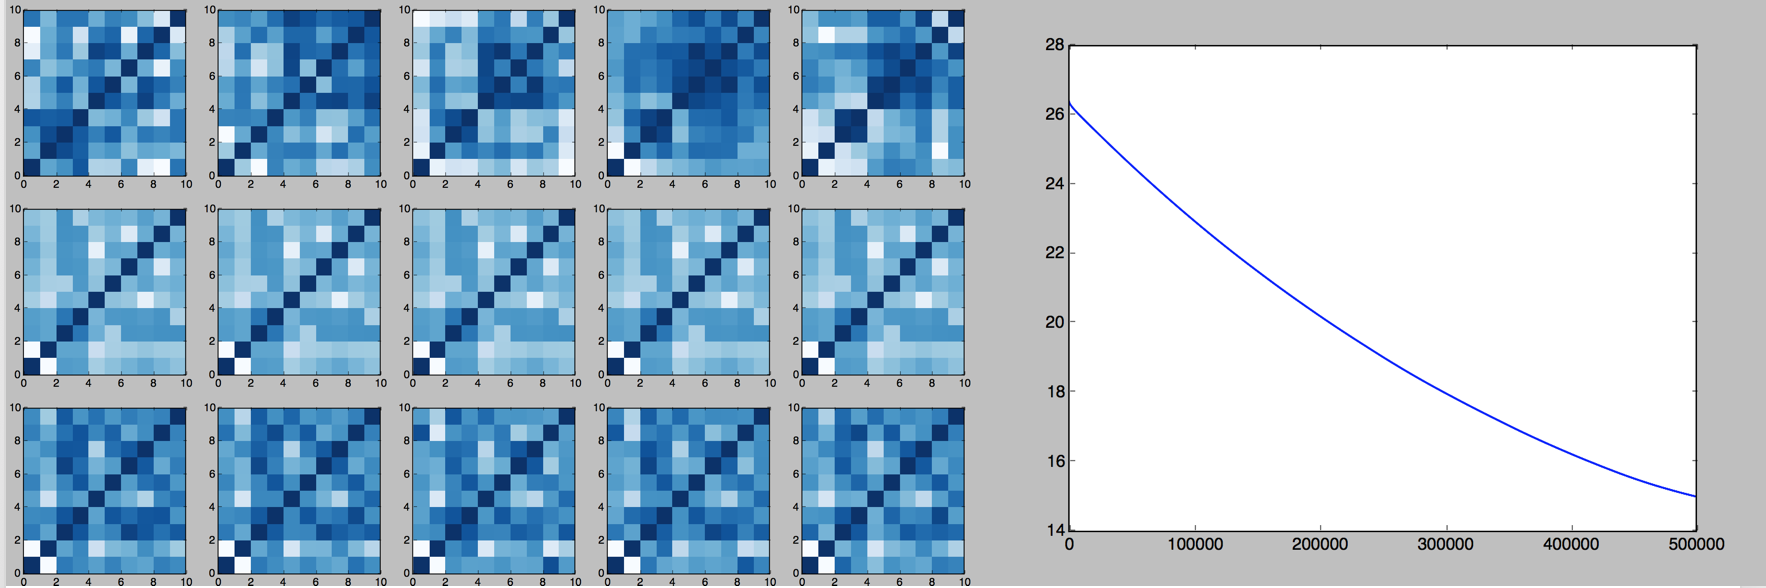
\includegraphics[width=.9\textwidth]{GaussianProcess.png}
\label{fig:gaussian}
\end{figure}
The rows in the left graph, from top to bottom, represent the ground truth covariances. the initializations and the recovered covariances, respectively; the columns, time points from 1 to 5. The graph on the right shows the value of the negative log-likelihood function over number of iterations.\par

From the right graph, we can see that MGP, through the process of optimizing the feature vectors and in extension the dynamic covariances, increases the likelihood (decreasing the negative log-likelihood) of the model. This is further confirmed from the results in the left graph. Comparing with the initializations, the recovered covariances objectively show more resemblance to the ground truth. However, when looking across all the time points, the recovered covariances looks very similar throughout the time sequence, without any distinctive features that could differentiate one time point from another. This is due to the Bayesian nature of MGP, by which the optimization process seeks to find the most probable covariance at each time point. However, as the ground truth is not always the point of highest probability on the distribution, MGP falls short of TimeCorr with respect to covariance recovery accuracy.\par

In addition, throughout the hundreds of test cases we went through, we discovered that MGP is prone to being stuck in local minimums. This problem is further exacerbated when we increase the number of variables, time points and feature length. As the dimensionality of the dataset increases, the probability space becomes increasingly more complex and more difficult to optimize on, and thus the likelihood sometimes sees minimal improvement over thousands of iterations.\par

Framing dynamic covariance recovery as a MGP optimization problem also increases the demand for computing resources. Even with only 5 time points, the MGP model takes 10-100 times longer to converge to a decent result than a TimeCorr model with 1000 time points. Furthermore, like most other Machine Learning models, it is very difficult to find the optimal configuration for optimization of the MGP model.\par

Lastly, selection of the kernel function is a very important factor when applying the MGP Model. Different data patterns correspond to very different kernel functions. Thus, correct application of the MGP Model also requires prior knowledge of the structure of the dataset.\par


\subsection{TimeCorr and Naive TimeCorr}
To compare the performance of TimeCorr and Naive TimeCorr, we generated three different datasets, all of which has Gaussian Variance=1000, Number of Time points=1000 and Number of Variables=5, to highlight TimeCorr's superiority in consistency and local accuracy:
\begin{enumerate}
\item A validation dataset with a constant covariance matrix $C$ for all time points, and a random unrelated covariance matrix for comparison. The results are displayed in Figure \ref{fig:validation}\par
\begin{figure}[h]
\caption{Validation Correlation: Ground Truth (solid); Random (dotted)}
\centering
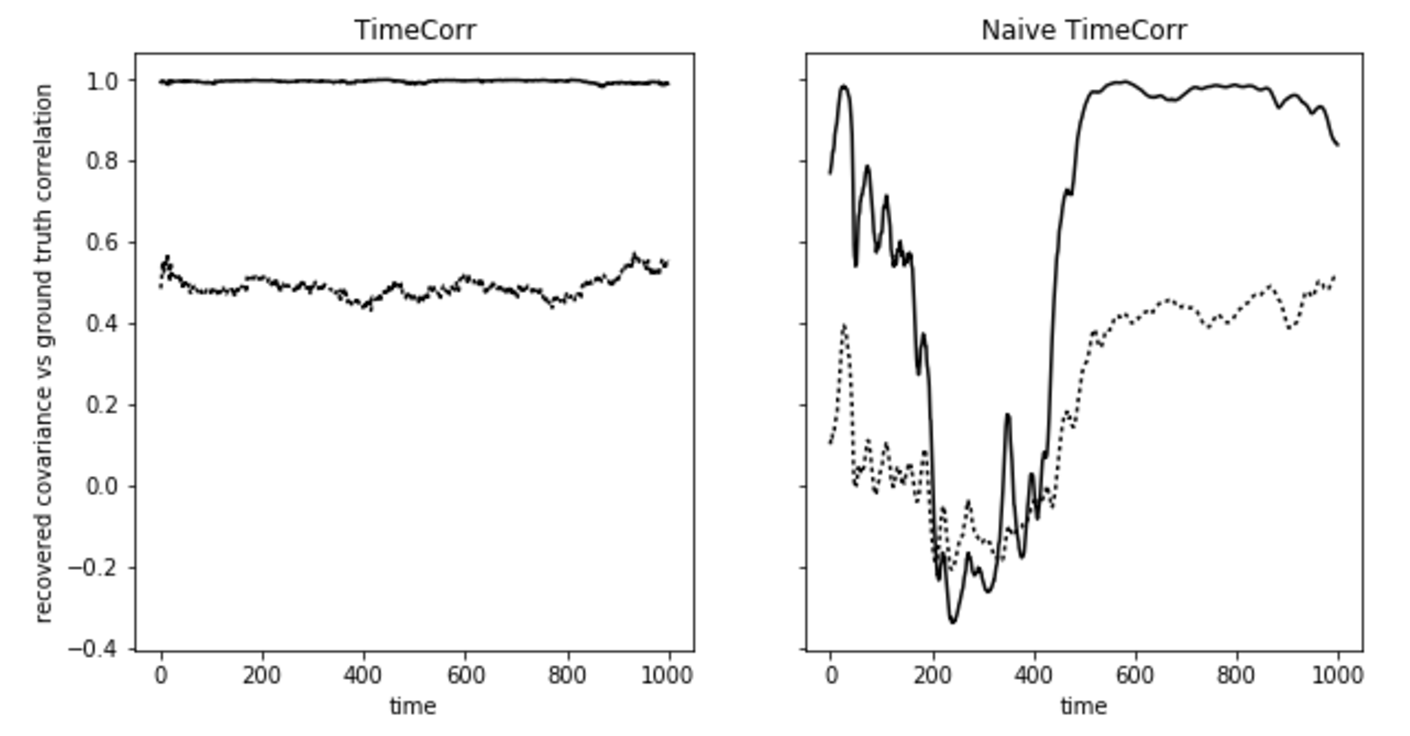
\includegraphics[width=0.7\textwidth]{ValidationComparison.png}
\label{fig:validation}
\end{figure}
From Figure \ref{fig:validation}, we can see that recovery from TimeCorr is highly consistent and robust across all time points. In addition, TimeCorr also creates greater distinction between dissimilar covariances. Furthermore, TimeCorr appears to be immune to the irregularities that is manifested by the Naive TimeCorr method\par

\item A fading dataset with dynamic covariance $C_t$ as a combination of one covariance $C_1$ linearly fading into another covariance $C_2$, where $C_t = \frac{1000-t}{1000}*C_1+\frac{t}{1000}*C_2$ at time point $t$. The results are displayed in Figure \ref{fig:fading}\par
\begin{figure}[h]
\caption{Fading Correlation: $C_1$ (solid), $C_2$ (dotted)}
\centering
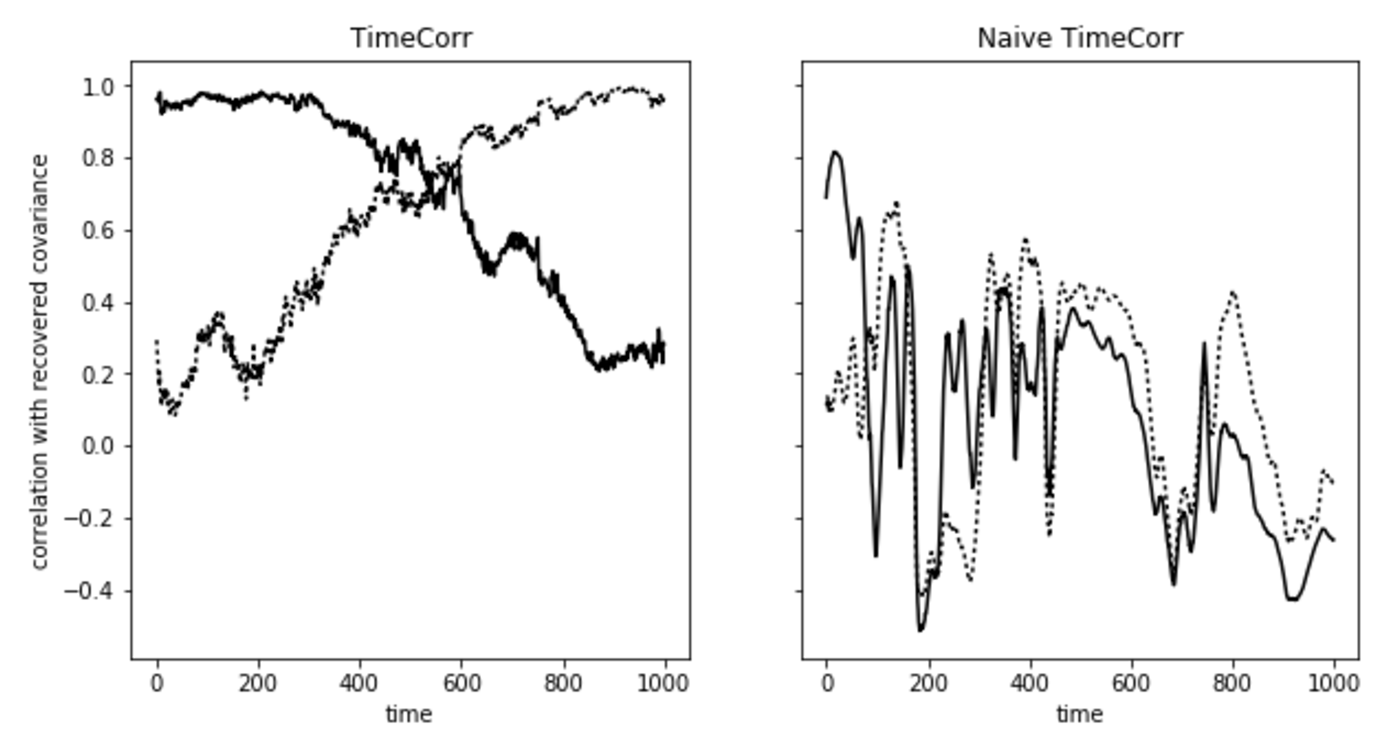
\includegraphics[width=0.9\textwidth]{FadingComparison.png}
\label{fig:fading}
\end{figure}
Figure \ref{fig:fading} shows the correlation between recovered dynamic covariances and ground truth. The TimeCorr approach is able to clearly recover the X shape that is to be expected of the correlations, whereas the Naive TimeCorr method is barely able to retrieve this pattern. From this comparison, we can see that TimeCorr is able to consistently recover dynamically changing covariances with very high accuracy, while results from the Naive TimeCorr method appear to be very inconsistent.

\item A cross dataset generated using $C_1$ as covariance for the first half, then abruptly changing to another covariance $C_2$ for the second half. The results are displayed in Figure \ref{fig:cross}\par
\begin{figure}[h]
\caption{Cross Correlation: $C_1$ (solid), $C_2$ (dotted)}
\centering
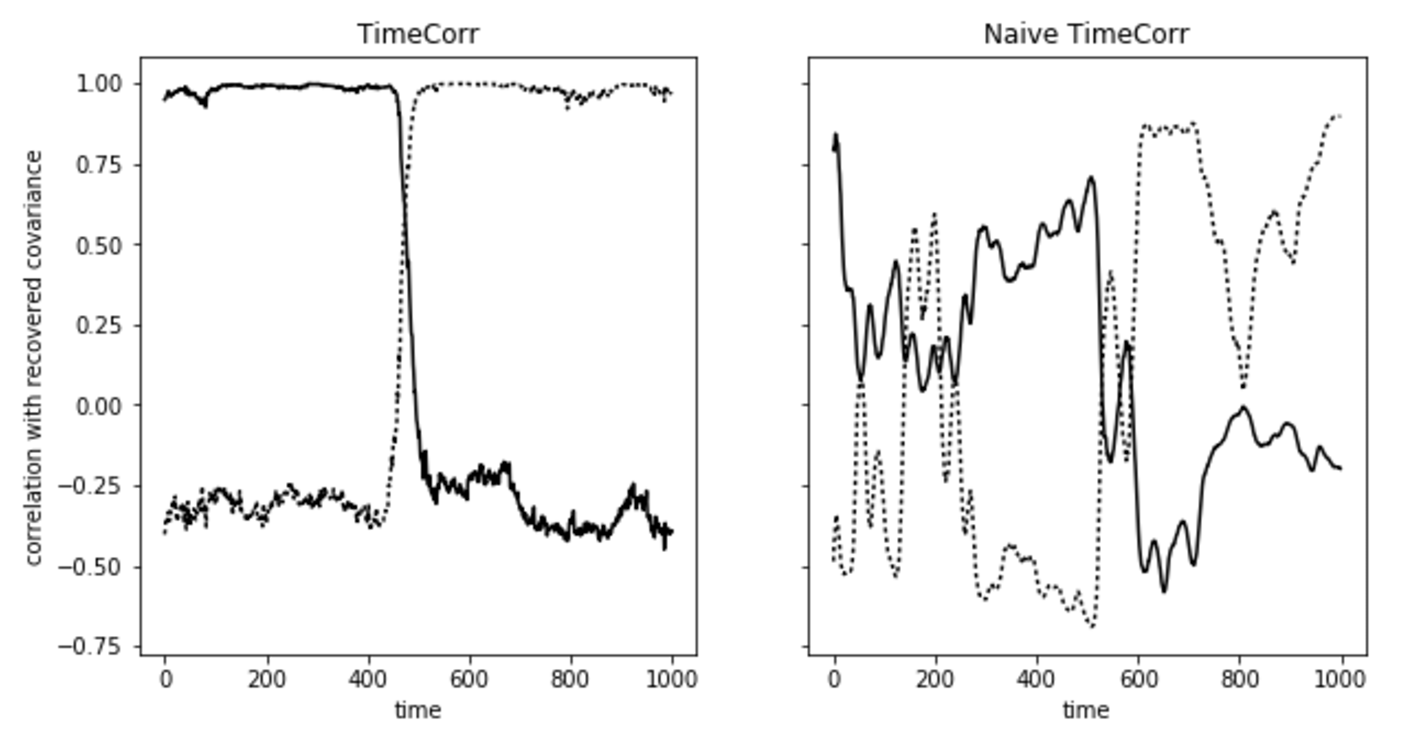
\includegraphics[width=0.8\textwidth]{CrossComparison.png}
\label{fig:cross}
\end{figure}
Figure \ref{fig:cross} displays the correlation between the recovered dynamic covariances and $C_1$ and $C_2$. As expected, the TimeCorr results remain consistently horizontal on the two ends of the graph, and distinctly and abruptly crosses at the midpoint. This behavior shows that the TimeCorr approach is robust to sudden changes in the covariance. In comparison, although the Naive TimeCorr method roughly displays the cross pattern, it is very inaccurate in estimation and generally very inconsistent.\par
\end{enumerate}

\subsection{More on TimeCorr}
To understand the full scope of capabilities of TimeCorr, we ran further tests using multiple configurations of varying Gaussian variances and Covariance Fragment Estimation Ranges (CFER)---the number of neighboring time points we use to calculate each covariance fragment. Through increasing the Gaussian variance of the Gaussian distribution behind the coefficients, the influence of a wider range of time points on the recovery process is increased. We expected that this will stabilize the results of our recovery even more. Following the same logic, we also explored different ranges for the CFER to see if higher values will also have stabilizing effects on our recovery.\par
In addition, to understand the limitations of TimeCorr, we attempted to use TimeCorr on multiple synthetic datasets that had dynamic covariances changing at increasingly rapid rates. As TimeCorr depends heavily on neighboring time points in the recovery of dynamic covariances, we suspected that TimeCorr will break down if the covariances change too fast.\par

\begin{enumerate}
\item Varying Gaussian Variance and comparing between TimeCorr and Naive TimeCorr\par
\begin{figure}[h]
\caption{Varying Gaussian Variance: TimeCorr vs Naive TimeCorr}
\centering
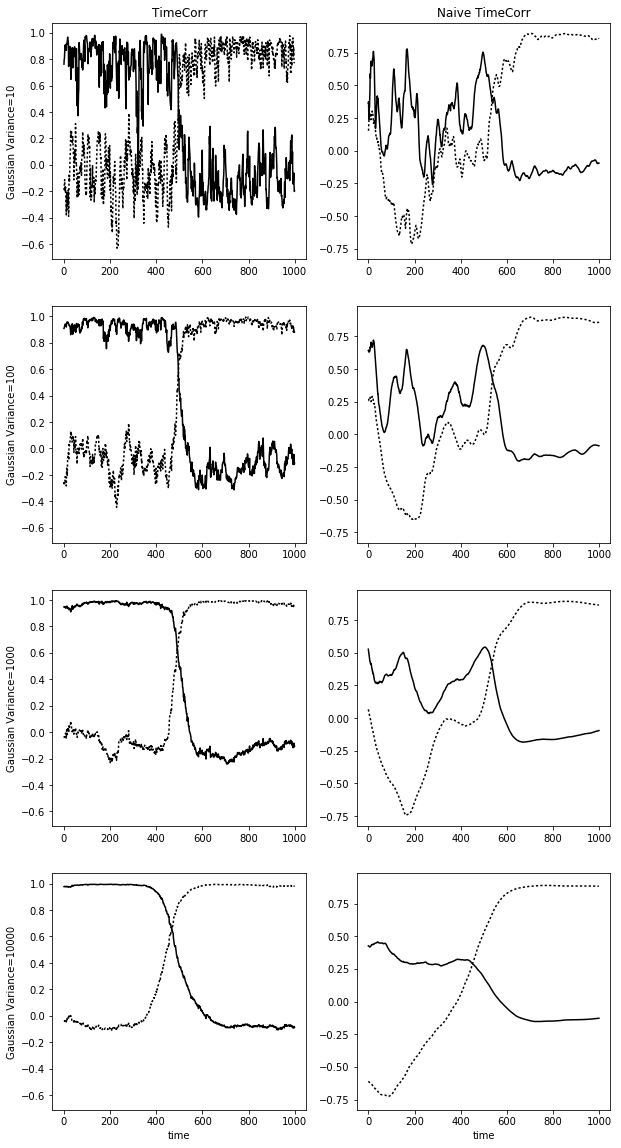
\includegraphics[width=0.5\textwidth]{VaryingGaussian1.png}
\label{fig:GaussianVariance}
\end{figure}
As the variance of the Gaussian distribution behind the coefficients increases, neighboring time points gain more influence. As a result, irregular fluctuations in the correlation are dampened and flattened. This effect is evident in results from both the TimeCorr and the Naive TimeCorr method. In Figure \ref{fig:GaussianVariance}, we can see that the expected X shape becomes more prominent as Gaussian Variance increases. At the same time, abrupt changes in the underlying dynamic covariance are dragged out into longer time frames in the recovered covariance from TimeCorr models with higher Gaussian Variance. For dynamic covariances that shifts slowly, this effect will stabilize the recovery process. But for dynamic covariances that changes rapidly, higher Gaussian variance may have adverse effects on the recovery.\par
\item Varying Gaussian Variance over a greater range, TimeCorr only\par
To further emphasize the effects of increasing Gaussian variance, we implemented TimeCorr on a cross dataset using Gaussian variances of 10, 100, 200, 500, 1000 and 10,000.\par
\begin{figure}[h]
\caption{Varying Gaussian Variance: focusing TimeCorr}
\centering
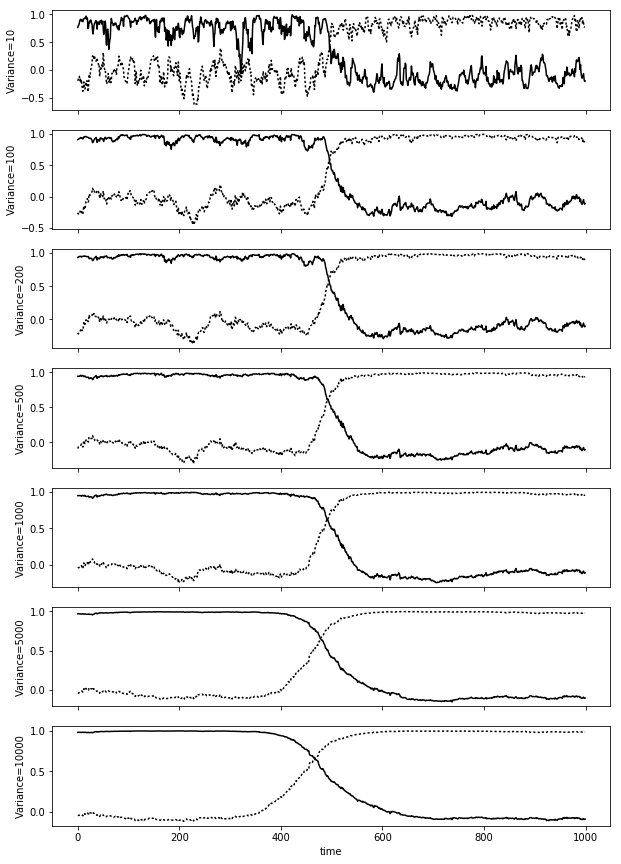
\includegraphics[width=0.5\textwidth]{VaryingGaussian2.png}
\label{fig:VaryingGaussian2}
\end{figure}
Consistent with our previous results, we see in Figure \ref{fig:VaryingGaussian2} that, as the Gaussian Variance increases, the curve becomes more smooth. However, the transition between the two covariances increases from 100 time points to almost 300 time points as Gaussian Variance increases from 10 to 10,000.\par
\item Varying Covariance Fragment Estimation Range (CFER), TimeCorr only\par
Another aspect of the TimeCorr that we explored is the length of the neighborhood that we use to calculate the covariance fragments---Covariance Fragment Estimation (CFER). We implemented TimeCorr on a cross dataset using CFER of 3, 11, 25, 51 and 101.\par
\begin{figure}[h]
\caption{Varying CFER}
\centering
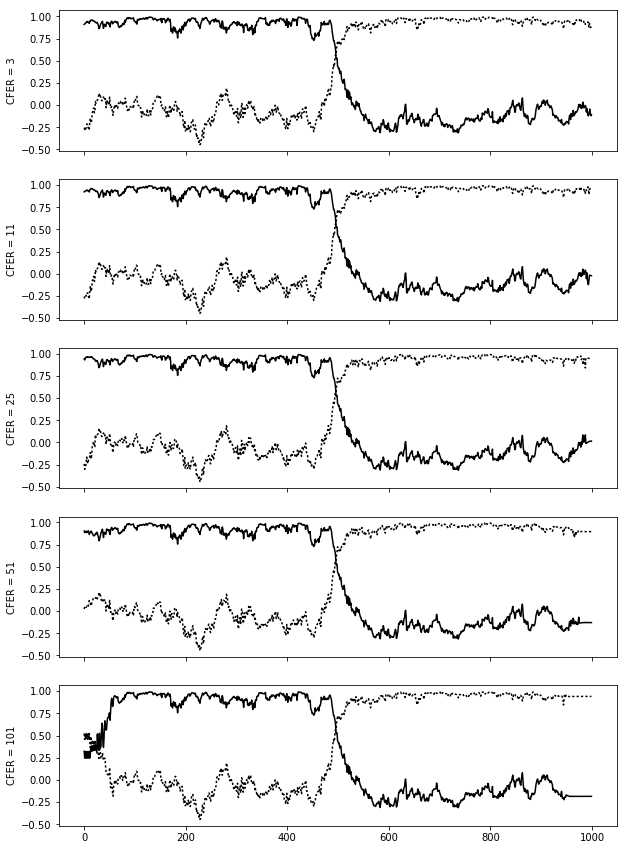
\includegraphics[width=0.5\textwidth]{VaryingCFER.png}
\label{fig:VaryingCFER}
\end{figure}
From Figure \ref{fig:VaryingCFER}, we see that there is not a huge difference in TimeCorr performance when using CFER of 3 to 25. However, as CFER increases beyond 51, we start to see abnormalities on the edges of the graphs. In addition, we suspect that TimeCorr models with large CFER values do not perform well on time sequence datasets with rapidly changing dynamic covariances. This is verified in the following section.\par
\item TimeCorr performance on time sequence data with rapidly changing covariance\par
Our first synthetic dataset was generated using 10 random covariances, each persisting for 100 time points before abruptly changing into another. For covariance recovery, we choose to use a TimeCorr model with Gaussian Variance=100 and CFER=3. The correlation between the recovered covariance and the true covariances are displayed in Figure \ref{fig:iteration10}, with each line representing correlation with a different true covariance.\par
\begin{figure}[h]
\caption{TimeCorr performance on dataset with 10 distinct covariances}
\centering
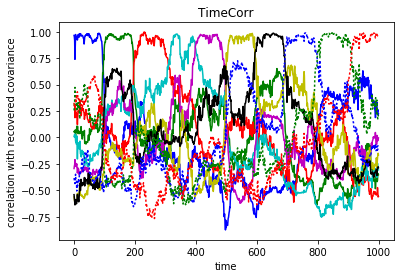
\includegraphics[width=0.5\textwidth]{iteration10.png}
\label{fig:iteration10}
\end{figure}
From Figure \ref{fig:iteration10}, we can see that the correlation between recovered covariance and the true covariances at each time point is distinctively higher than the correlation between recovered covariance and other covariances. For further testing and for better visualization, we used TimeCorr on 1000 time point synthetic datasets with 10, 25, 50, 100 and 250 covariances. The true covariances are indexed from 0 to [number of covariances-1], sequentially. The scatter plot shows the index of the true covariance that has the highest correlation with the recovered covariance at each time point. In the ideal scenario, the points should be distributed along the diagonal.\par
\begin{figure}[h]
\caption{TimeCorr performance with Variance=100 and CFER=3}
\centering
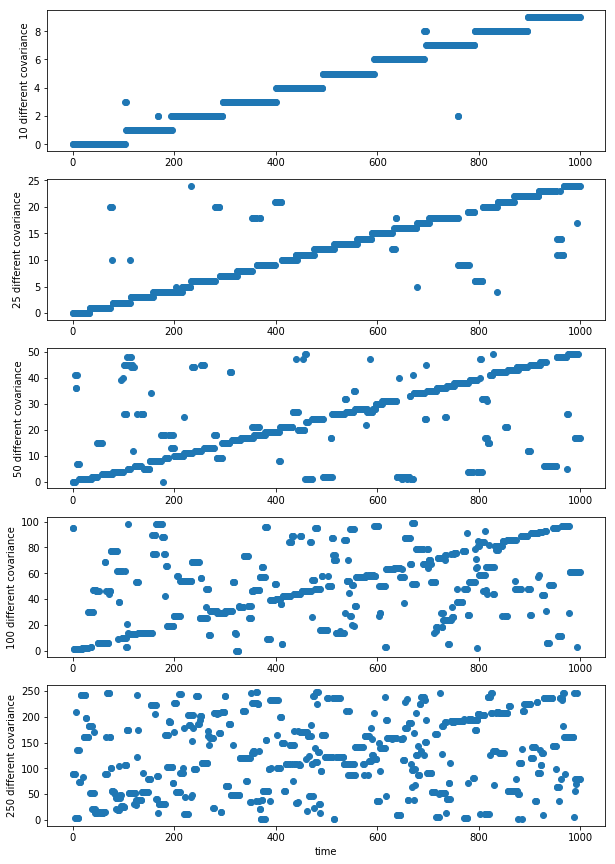
\includegraphics[width=0.7\textwidth]{scatter1003.png}
\label{fig:scatter1003}
\end{figure}
The average percentage of time points that the TimeCorr model with CFER of 3 was able to correctly recover from 10 repetitions per scenario was 94.3\%, 79.4\%, 52.2\%, 19.9\% and 5.2\% for datasets with 10, 25, 50, 100 and 250 distinct covariances, respectively. This is consistent from the results shown in Figure \ref{fig:scatter1003}, where the recovered covariances is consistently correct for datasets with slower changing dynamic covariances, but become more random for datasets whose underlying dynamic covariances change more rapidly. As the time spread of each distinct covariance approaches the Covariance Fragment Estimation Range, TimeCorr become increasingly less accurate. To further verify the inverse relationship between recovery accuracy and the difference between CFER and dataset covariance time interval, we changed CFER to 11 and received the results in Figure \ref{fig:scatter10011}.\par
\begin{figure}[h]
\caption{TimeCorr performance with Variance=100 and CFER=11}
\centering
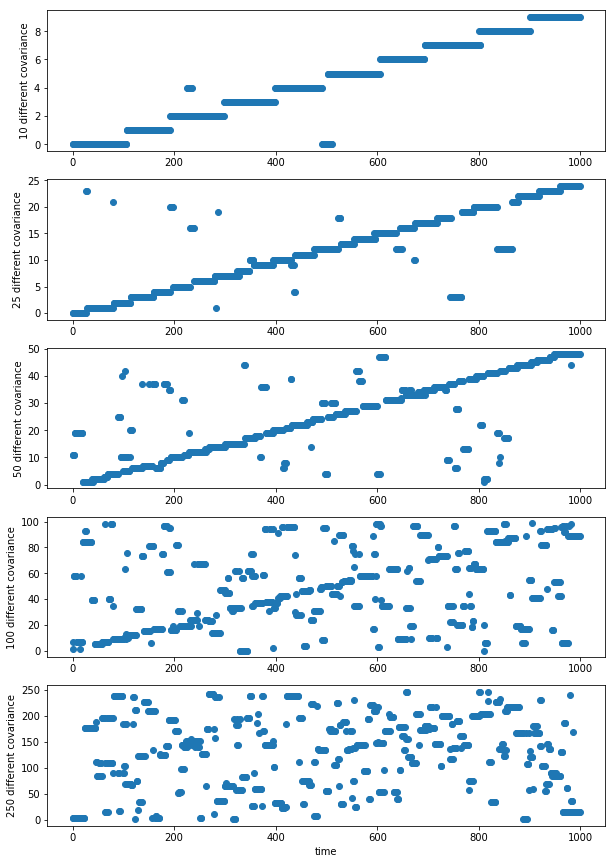
\includegraphics[width=0.5\textwidth]{scatter10011.png}
\label{fig:scatter10011}
\end{figure}
The average percentage of time points that the TimeCorr model with CFER of 11 was able to correctly recover from 10 repetitions per scenario was 94.6\%, 81.2\%, 58.3\%, 14.5\% and 3.1\% for datasets with 10, 25, 50, 100 and 250 distinct covariances, respectively. When the covariance time interval is greater than the CFER, the accuracy for the model with variance=100 and CFER=11 is consistently higher than that of the model with variance=100 and CFER=3---94.6\% vs 94.3\%, 81.2\% vs 79.4\%, 58.3\% vs 52.2\%---which means longer CFER produces higher recovery accuracy. However, when the covariance time interval = $\frac{1000}{100}=10$, the accuracy for the model with CFER=3$<$10 becomes significantly higher than that of the model with CFER=11$>$10, which proves that the recovery accuracy of TimeCorr is highly dependent on the CFER being shorter than the time interval each distinct covariance occupies.\par
Finally, to analyze the effect of Gaussian Variance on recovery accuracy, we conducted testing using a TimeCorr model with Variance=1000 and CFER=3. The results are show in \ref{fig:scatter10003}\par
\begin{figure}[h]
\caption{TimeCorr performance with Variance=1000 and CFER=3}
\centering
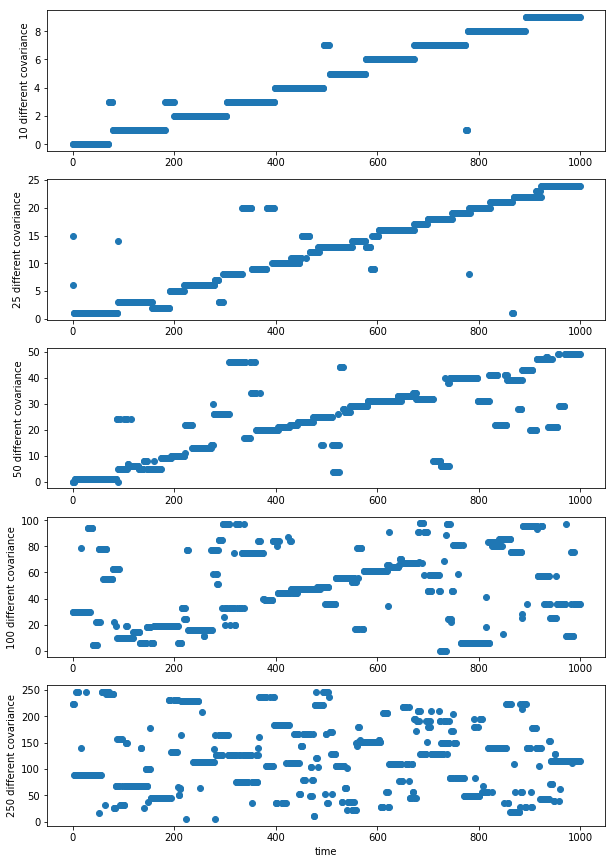
\includegraphics[width=0.5\textwidth]{scatter10003.png}
\label{fig:scatter10003}
\end{figure}
The average percentage of time points that TimeCorr was able to correctly recover from 10 repetitions per scenario was 84.7\%, 49\%, 19.9\%, 7.8\% and 1\% for datasets with 10, 25, 50, 100 and 250 distinct covariances, respectively. The results were consistently worse that that of the TimeCorr model with Gaussian Variance=100. This is also evident qualitatively as the results in Figure \ref{fig:scatter10003} appears to be much more random than that of Figure \ref{fig:scatter1003}. Therefore, we conclude that smaller Gaussian Variance produces higher recovery accuracy on datasets with rapidly changing dynamic covariances\par



\end{enumerate}

\section{Conclusion}
In conclusion, we demonstrated that the TimeCorr model performs significantly better than both the Naive TimeCorr model and the Multivariate Gaussian model across all of our test cases. Specifically, the TimeCorr method
\begin{enumerate}
\item takes up significantly less computing resources when comparing with the Multivariate Gaussian Model
\item achieves more accurate and consistent recovery of the dynamic covariances at every time point
\item is more sensitive to both gradual and abrupt changes in the dynamic covariances
\item is very simple and intuitive, and very easy to configure
\end{enumerate}
In addition, to maximize dynamic covariance recovery accuracy of time sequence data, it is important to:
\begin{enumerate}
\item select proper Covariance Fragment Estimation Range (CFER) that is short enough to capture the rate of change of the dynamic covariance, but also large enough to maximize accuracy
\item select proper Gaussian Variance that is proportional to the size of the dataset
\end{enumerate}

\textbf{Next Steps}\par
As recovery of dynamic covariances in time sequence data is a very general problem that exists in many different fields---Brain Science, Finance, Economics, Biology, Mathematics, etc---we hope to organize this method into a toolbox and make it available for the general public.\par
In addition, the development of the TimeCorr model was conceived as an answer to the demand from the Contextual Dynamics Laboratory to recover the dynamic covariances within the fRMI data. We are excited to see what kind of interesting patterns we can obtain when we incorporate the TimeCorr model in analysis of the human brain.\par

\newpage
\section{Appendix}
\begin{enumerate}
\item \textbf{Likelihood Function}
\begin{align*}
L(a|f)&= \sum_t P(f_t)P(a_t|f_t)\\
 &\sim \sum_t  \log [P(f_t)P(a_t|f_t)]\\
&=\sum_t[ \log P(f_t)+\log P(a_t|f_t)]\\
&=\sum_t [-\frac12(a_t^TC_t^{-1}a_t)-\frac12\log\det(C_t)+\log P(f_t)]\\
&=\sum_t [-\frac12 (a_t^TC_t^{-1}a_t)-\frac12\log||C^t||+\log[\exp(-\frac{f_0^2}{2\sigma_0^2})\prod_t\exp(-\frac{(f_t-f_{t-1})^2}{2\sigma_{t-1}^2})]\\
&=\sum_t[-\frac12 (a_t^TC_t^{-1}a_t)-\frac12\log||C_t||-\frac{f_0^2}{2\sigma_0^2}-\sum_t\frac{(f_t-f_{t-1})^2}{2\sigma_{t-1}^2}]\\
\end{align*}
\item \textbf{Multivariate Gaussian Process Gradient Derivation}\par
Feature $k$ of variable $i$ at time $t$ is represented by $f_t^{ik}$. The gradient of the likelihood function with respect to $f_t^{ik}$ is:
\begin{align*}
\nabla_{f_t^{ik}} L(a|f) &= \argmax_{f^{ik}_t} P(f_t)P(a_t|f_t) \\
&=\argmax_{f_t^{ik}} [\log P(f_t)+\log P(a_t|f_t)]\\
&=\argmax_{f_t^{ik}}[-\frac12 (a_t^TC_t^{-1}a_t)-\frac12\log||C_t||-\frac{(f_0^{ik})^2}{2\sigma_0^2}-\sum_t\frac{(f_t^{ik}-f^{ik}_{t-1})^2}{2\sigma_{t-1}^2}]
\end{align*}
\vspace{5mm}
To find the optimal features that maximizes this probability, we take the derivative:
\begin{align*}
\frac{\delta [P(f_t)P(a_t|f_t)]}{\delta f_{t}^{ik}}&=\begin{cases}
\frac12a_t^TC_t^{-1}\frac{\delta C_t}{\delta f_{t}^{ik}}C_t^{-1}a_t-\frac12 \tr(C_t^{-1}\frac{\delta C_t}{\delta f_{t}^{ik}})-\frac{f_{t}^{ik}}{\sigma_0^2} \text{ for } t=0\\
\\
 \frac12a_t^TC_t^{-1}\frac{\delta C_t}{\delta f_{t}^{ik}}C_t^{-1}a_t-\frac12 \tr(C_t^{-1}\frac{\delta C_t}{\delta f_{t}^{ik}})-\frac{f_{t}^{ik}-f_{t-1}^{ik}}{\sigma_{t-1}^2} \text{ for } t\neq0\\
 \end{cases}
\end{align*}
\vspace{5mm}
Setting $\alpha_t = C_t^{-1} a_t$ and simplifying:
\begin{align*}
\frac{\delta [P(f_t)P(a_t|f_t)]}{\delta f_{t}^{ik}}&=\begin{cases}
\frac12\tr[(\alpha_t^T\alpha_t-C_t^{-1})\frac{\delta C_t}{\delta f_{t}^{ik}}]-\frac{f_{t}^{ik}}{\sigma_0^2}\text{ for } t=0\\
\\
 \frac12\tr[(\alpha_t^T\alpha_t-C_t^{-1})\frac{\delta C_t}{\delta f_{t}^{ik}}]-\frac{f_{t}^{ik}-f_{t-1}^{ik}}{\sigma_{t-1}^2} \text{ for } t\neq0\\
 \end{cases}
\end{align*}
\vspace{5mm}
Given kernel function for the covariance matrix:
\begin{align*}
C_t^{ij}=K(f_t^i,f_t^j)=2 \exp(-\frac{||f_t^i-f_t^j||^2}{2\sigma_k^2})-1 \
\end{align*}
The derivative of covariance matrix $C_t$ with respect to feature $f_t^{ik}$ becomes zero except for row j and column j, where it takes the value of:
\begin{align*}
\frac{\delta C_{t}^{ij}}{\delta f_{t}^{ik}} = -\frac{2(f_{t}^{ik}-f_{t}^{jk})}{\sigma_k^2}\exp(-\frac{||f_{t}^i-f_{t}^j||^2}{2\sigma_k^2})
\end{align*}
*Part of this derivation comes from Murphy's "Machine Learning: A Probabilistic Perspective" \cite{murphy}


\newpage
\begin{thebibliography}{1}
\bibitem{murphy} Murphy, Kevin P "Gaussian Process." Machine Learning: A Probabilistic Perspective. 2012: MIT Press.
\end{thebibliography}
\end{enumerate}
\end{document}
